\pagebreak
\subsection{Adaptive Iterations}
%[15\%] Perform adaptive iterations for $\alpha = [0.5, 1, 1.5, 2, 2.5, 3]$ degrees. Run the same number of adaptive iterations for each $\alpha$ at least 5. Plot the ATPR output from your finest mesh versus alpha, and discuss the trend. Include flowfield plots to augment your discussion.

In the final section, I will vary the angle of attack as well as performing adaptive mesh refinements to determine the effects of $\alpha$ on the Mach field plot, the total pressure field plot, and the ATPR output. 

\subsubsection{ATPR Versus Angle of Attack}
\begin{figure}[h]
    \centering
    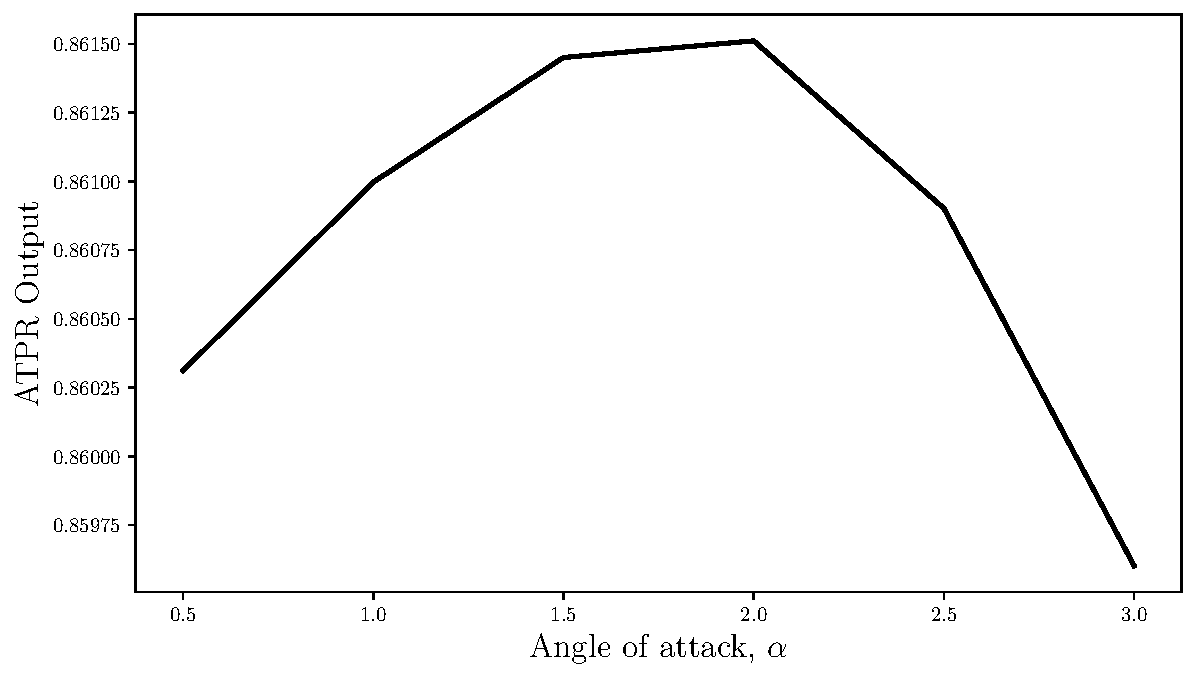
\includegraphics[width = 0.9\linewidth]{rep/q5/ATPR.pdf}
    \caption[ATPR and Angle of Attack]{Effects of varying $\alpha$ on the ATPR output.}
    \label{fig:aoa_ATPR}
\end{figure}

Shown above in Figure \ref{fig:aoa_ATPR}, is the effect of varying the angle of attack on ATPR output. In this analysis there is not a significant difference in the ATPR output while varying the angle of attack but there is a difference nonetheless. This difference in ATPR is causes from the flow hitting different incident angles along the contour of the nozzle inlet resulting in different flow patterns within the nozzle. Looking to Table \ref{tab:ATPR_alpha}, below for a Python print out of the values shown above for more accuracy.

\begin{table}[h]
    \centering
    \caption[ATPR Versus Angle of Attack]{ATPR versus angle of attack $\alpha$.}
    \label{tab:ATPR_alpha}
    \begin{tabular}{l|l}
        $\alpha$ & ATPR\\ \hline\hline
        \input{rep/q5/atpr_out}
    \end{tabular}
\end{table}

\pagebreak
\subsubsection{Flow Fields for Varying Angle of Attacks}
\begin{figure}[h]
    \centering
    \begin{subfigure}[h]{0.48\linewidth}
        \centering
        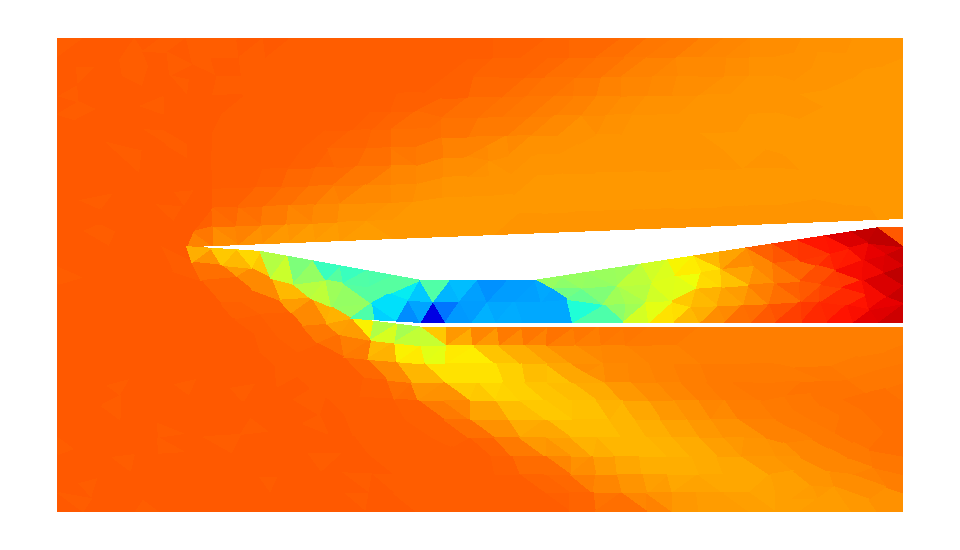
\includegraphics[width=\linewidth]{rep/q5/mach_a5.pdf}
        \caption{Mach field at $\alpha=0.5\degree$.}
    \end{subfigure}
    \begin{subfigure}[h]{0.48\linewidth}
        \centering
        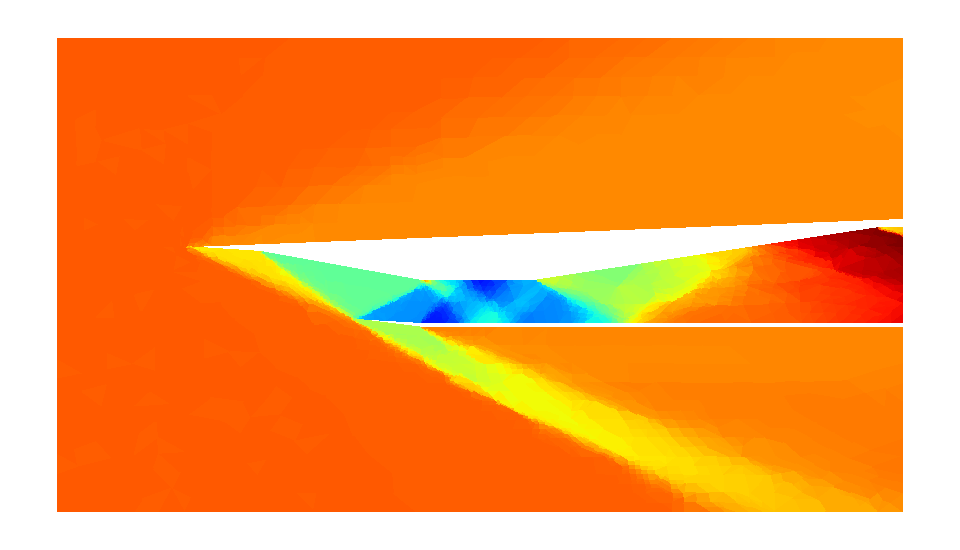
\includegraphics[width=\linewidth]{rep/q5/mach_a10.pdf}
        \caption{Mach field at $\alpha=1.0\degree$.}
    \end{subfigure}

    \begin{subfigure}[h]{0.48\linewidth}
        \centering
        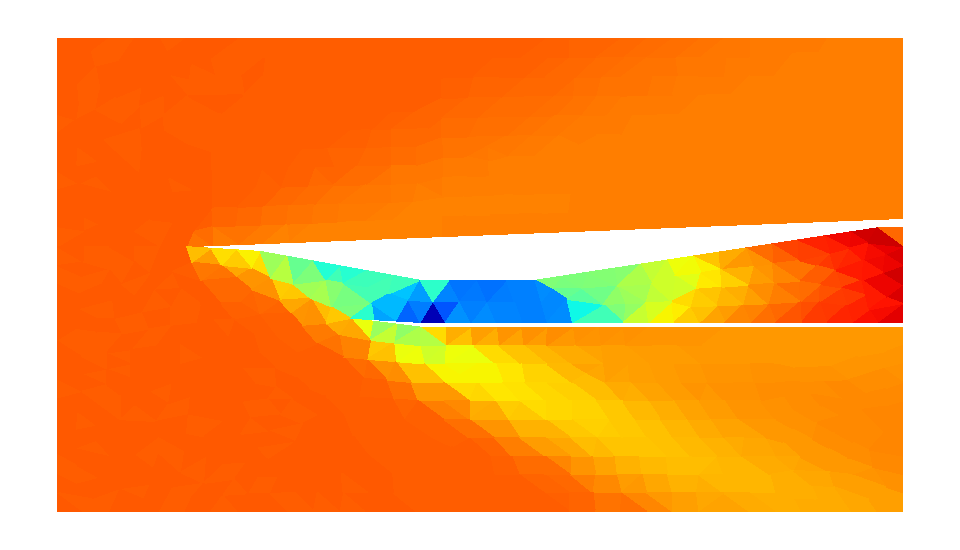
\includegraphics[width=\linewidth]{rep/q5/mach_a15.pdf}
        \caption{Mach field at $\alpha=1.5\degree$.}
    \end{subfigure}
    \begin{subfigure}[h]{0.48\linewidth}
        \centering
        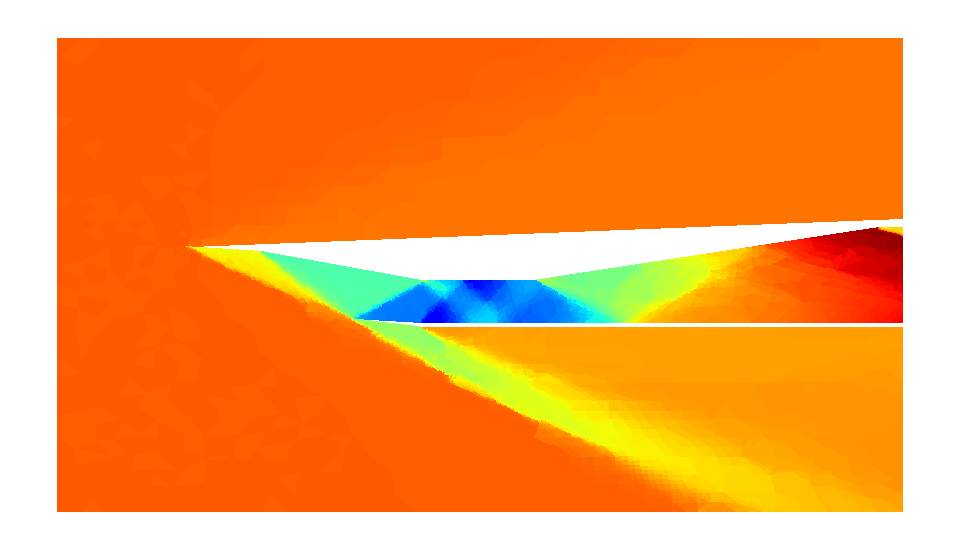
\includegraphics[width=\linewidth]{rep/q5/mach_a20.pdf}
        \caption{Mach field at $\alpha=2.0\degree$.}
    \end{subfigure}

    \begin{subfigure}[h]{0.48\linewidth}
        \centering
        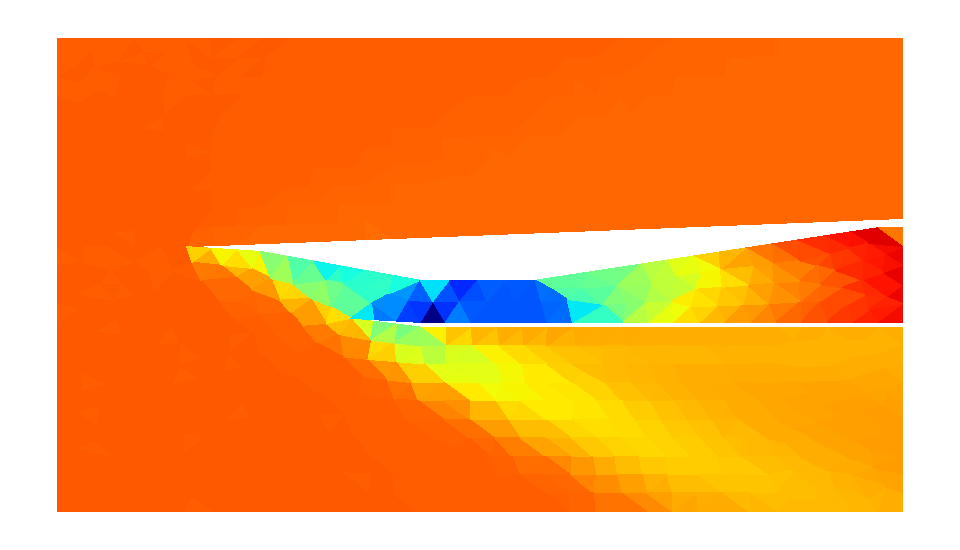
\includegraphics[width=\linewidth]{rep/q5/mach_a25.pdf}
        \caption{Mach field at $\alpha=2.5\degree$.}
    \end{subfigure}
    \begin{subfigure}[h]{0.48\linewidth}
        \centering
        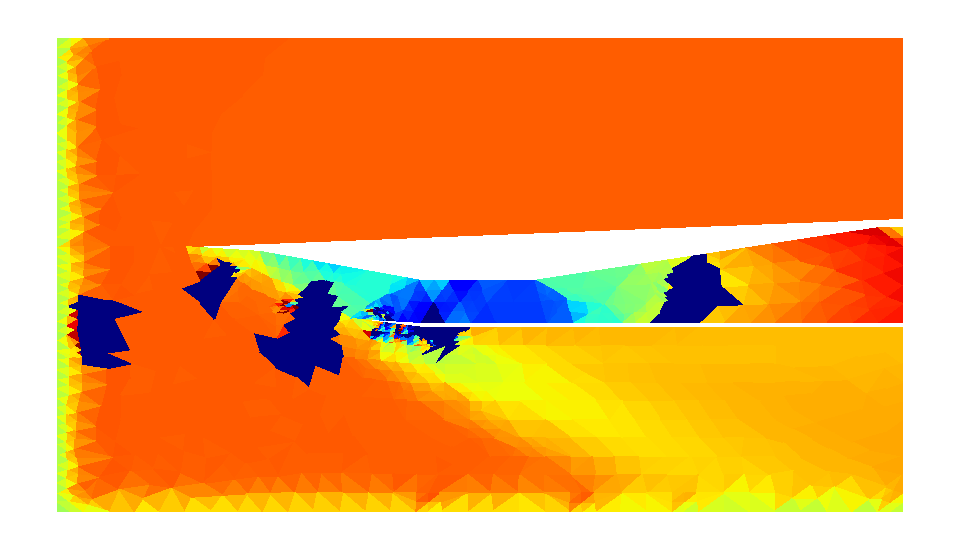
\includegraphics[width=\linewidth]{rep/q5/mach_a30.pdf}
        \caption{Mach field at $\alpha=3.0\degree$.}
    \end{subfigure}
    \caption[Mach Field with Varying Angle of Attack]{Varying angle of attack, and its effect on the mach field.}
    \label{fig:mach_fields}
\end{figure}

\paragraph{Effect on Mach Field from Varying Angle of Attack} Shown above in Figure \ref{fig:mach_fields} are the Mach fields for varying angles of attack. As shown above, there is not a large difference between the angle of attack configurations, but there are minor differences that can be spotted along the interior of the engine inlet. This is caused from the angle of attack hitting different incident angles and changing the flow pattern.

\pagebreak
\begin{figure}[h]
    \centering
    \begin{subfigure}[h]{0.48\linewidth}
        \centering
        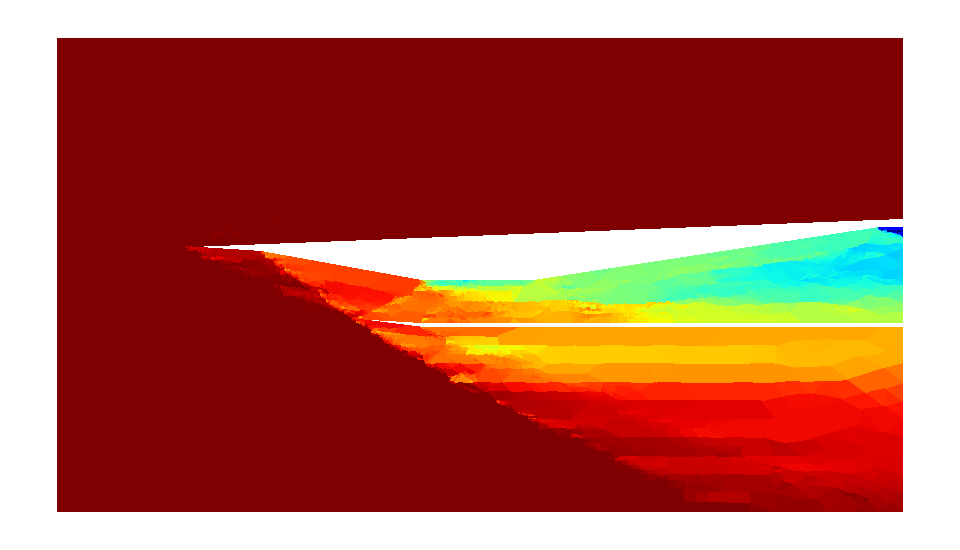
\includegraphics[width=\linewidth]{rep/q5/pt_a5.pdf}
        \caption{Total pressure field at $\alpha=0.5\degree$.}
    \end{subfigure}
    \begin{subfigure}[h]{0.48\linewidth}
        \centering
        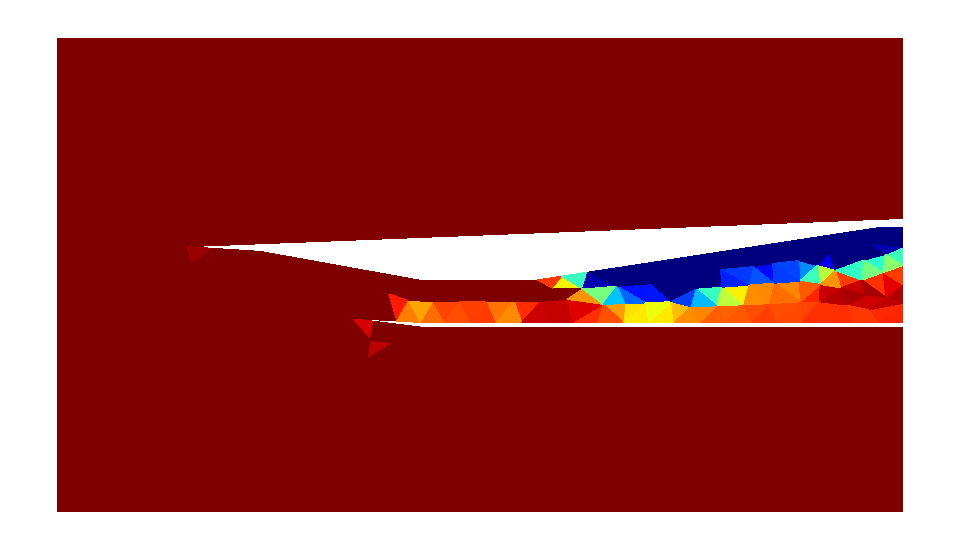
\includegraphics[width=\linewidth]{rep/q5/pt_a10.pdf}
        \caption{Total pressure field at $\alpha=1.0\degree$.}
    \end{subfigure}

    \begin{subfigure}[h]{0.48\linewidth}
        \centering
        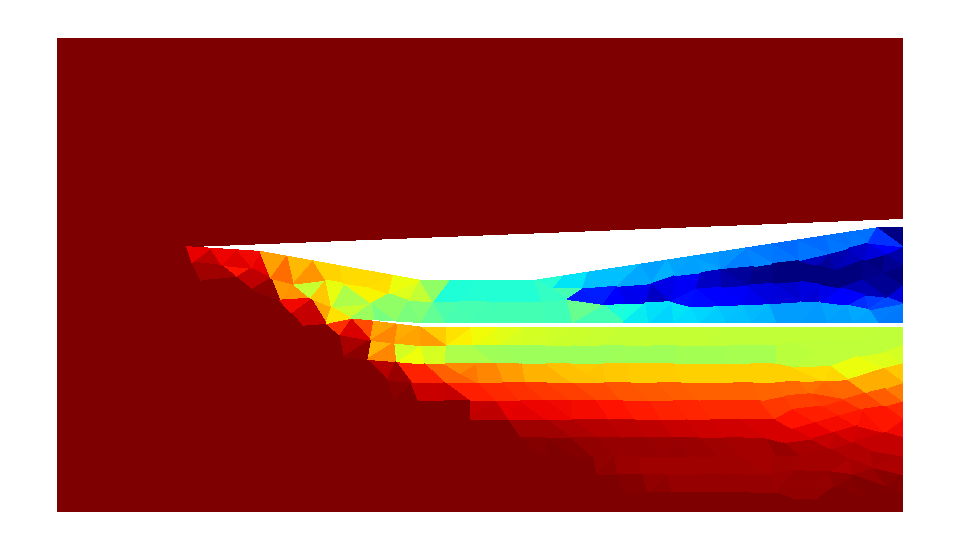
\includegraphics[width=\linewidth]{rep/q5/pt_a15.pdf}
        \caption{Total pressure field at $\alpha=1.5\degree$.}
    \end{subfigure}
    \begin{subfigure}[h]{0.48\linewidth}
        \centering
        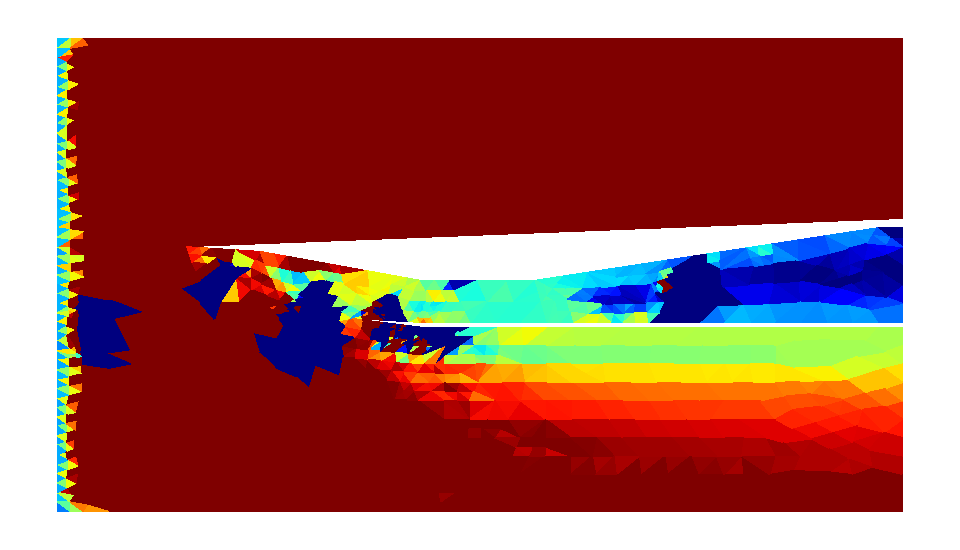
\includegraphics[width=\linewidth]{rep/q5/pt_a20.pdf}
        \caption{Total pressure field at $\alpha=2.0\degree$.}
    \end{subfigure}

    \begin{subfigure}[h]{0.48\linewidth}
        \centering
        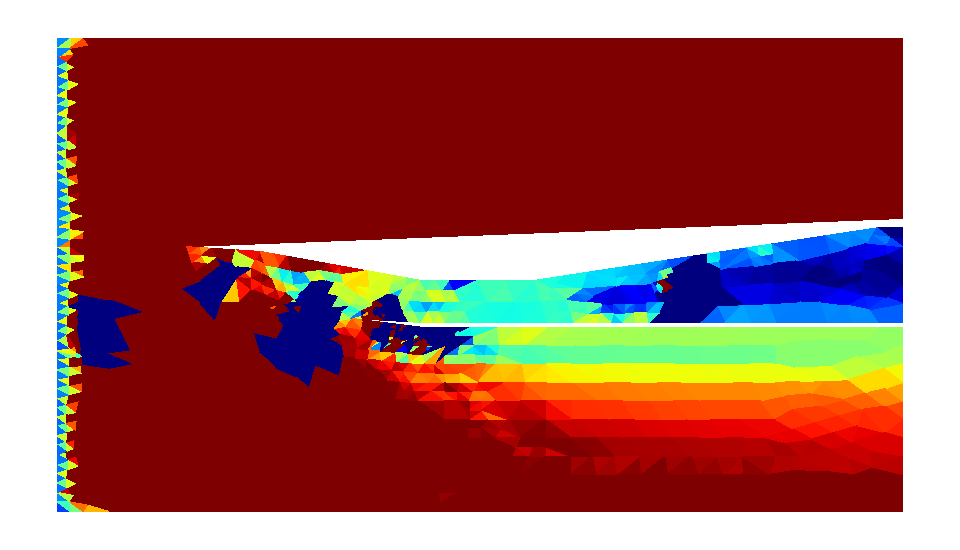
\includegraphics[width=\linewidth]{rep/q5/pt_a25.pdf}
        \caption{Total pressure field at $\alpha=2.5\degree$.}
    \end{subfigure}
    \begin{subfigure}[h]{0.48\linewidth}
        \centering
        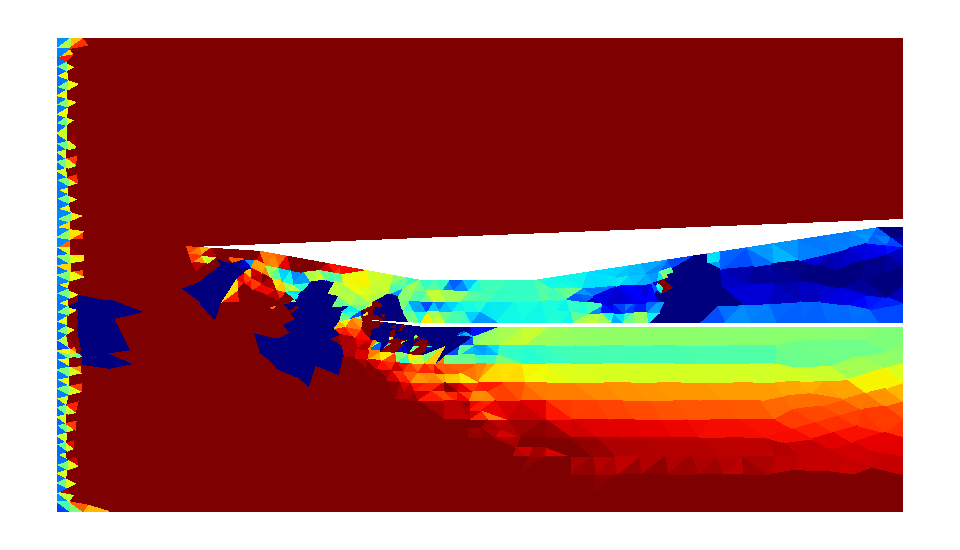
\includegraphics[width=\linewidth]{rep/q5/pt_a30.pdf}
        \caption{Total pressure field at $\alpha=3.0\degree$.}
    \end{subfigure}
    \caption[Total Pressure Field with Varying Angle of Attack]{Varying angle of attack, and its effect on the total pressure field.}
    \label{fig:pt_fields}
\end{figure}

\paragraph{Effect on Total Pressure Field from Varying Angle of Attack} Shown above in Figure \ref{fig:pt_fields} are the total pressure fields for varying angles of attack. In this analysis, there is not a large difference (at least not as much as the Mach field), which alters the total pressure within the nozzle. However, the most notable difference will be the total pressure below the engine cause by a larger stagnation of pressure due to the increased angle of attack.


